\appendix
% \section*{APPENDICES}
\renewcommand{\thesection}{Appendix \Alph{section}}

\begin{figure}[t!]
\centering
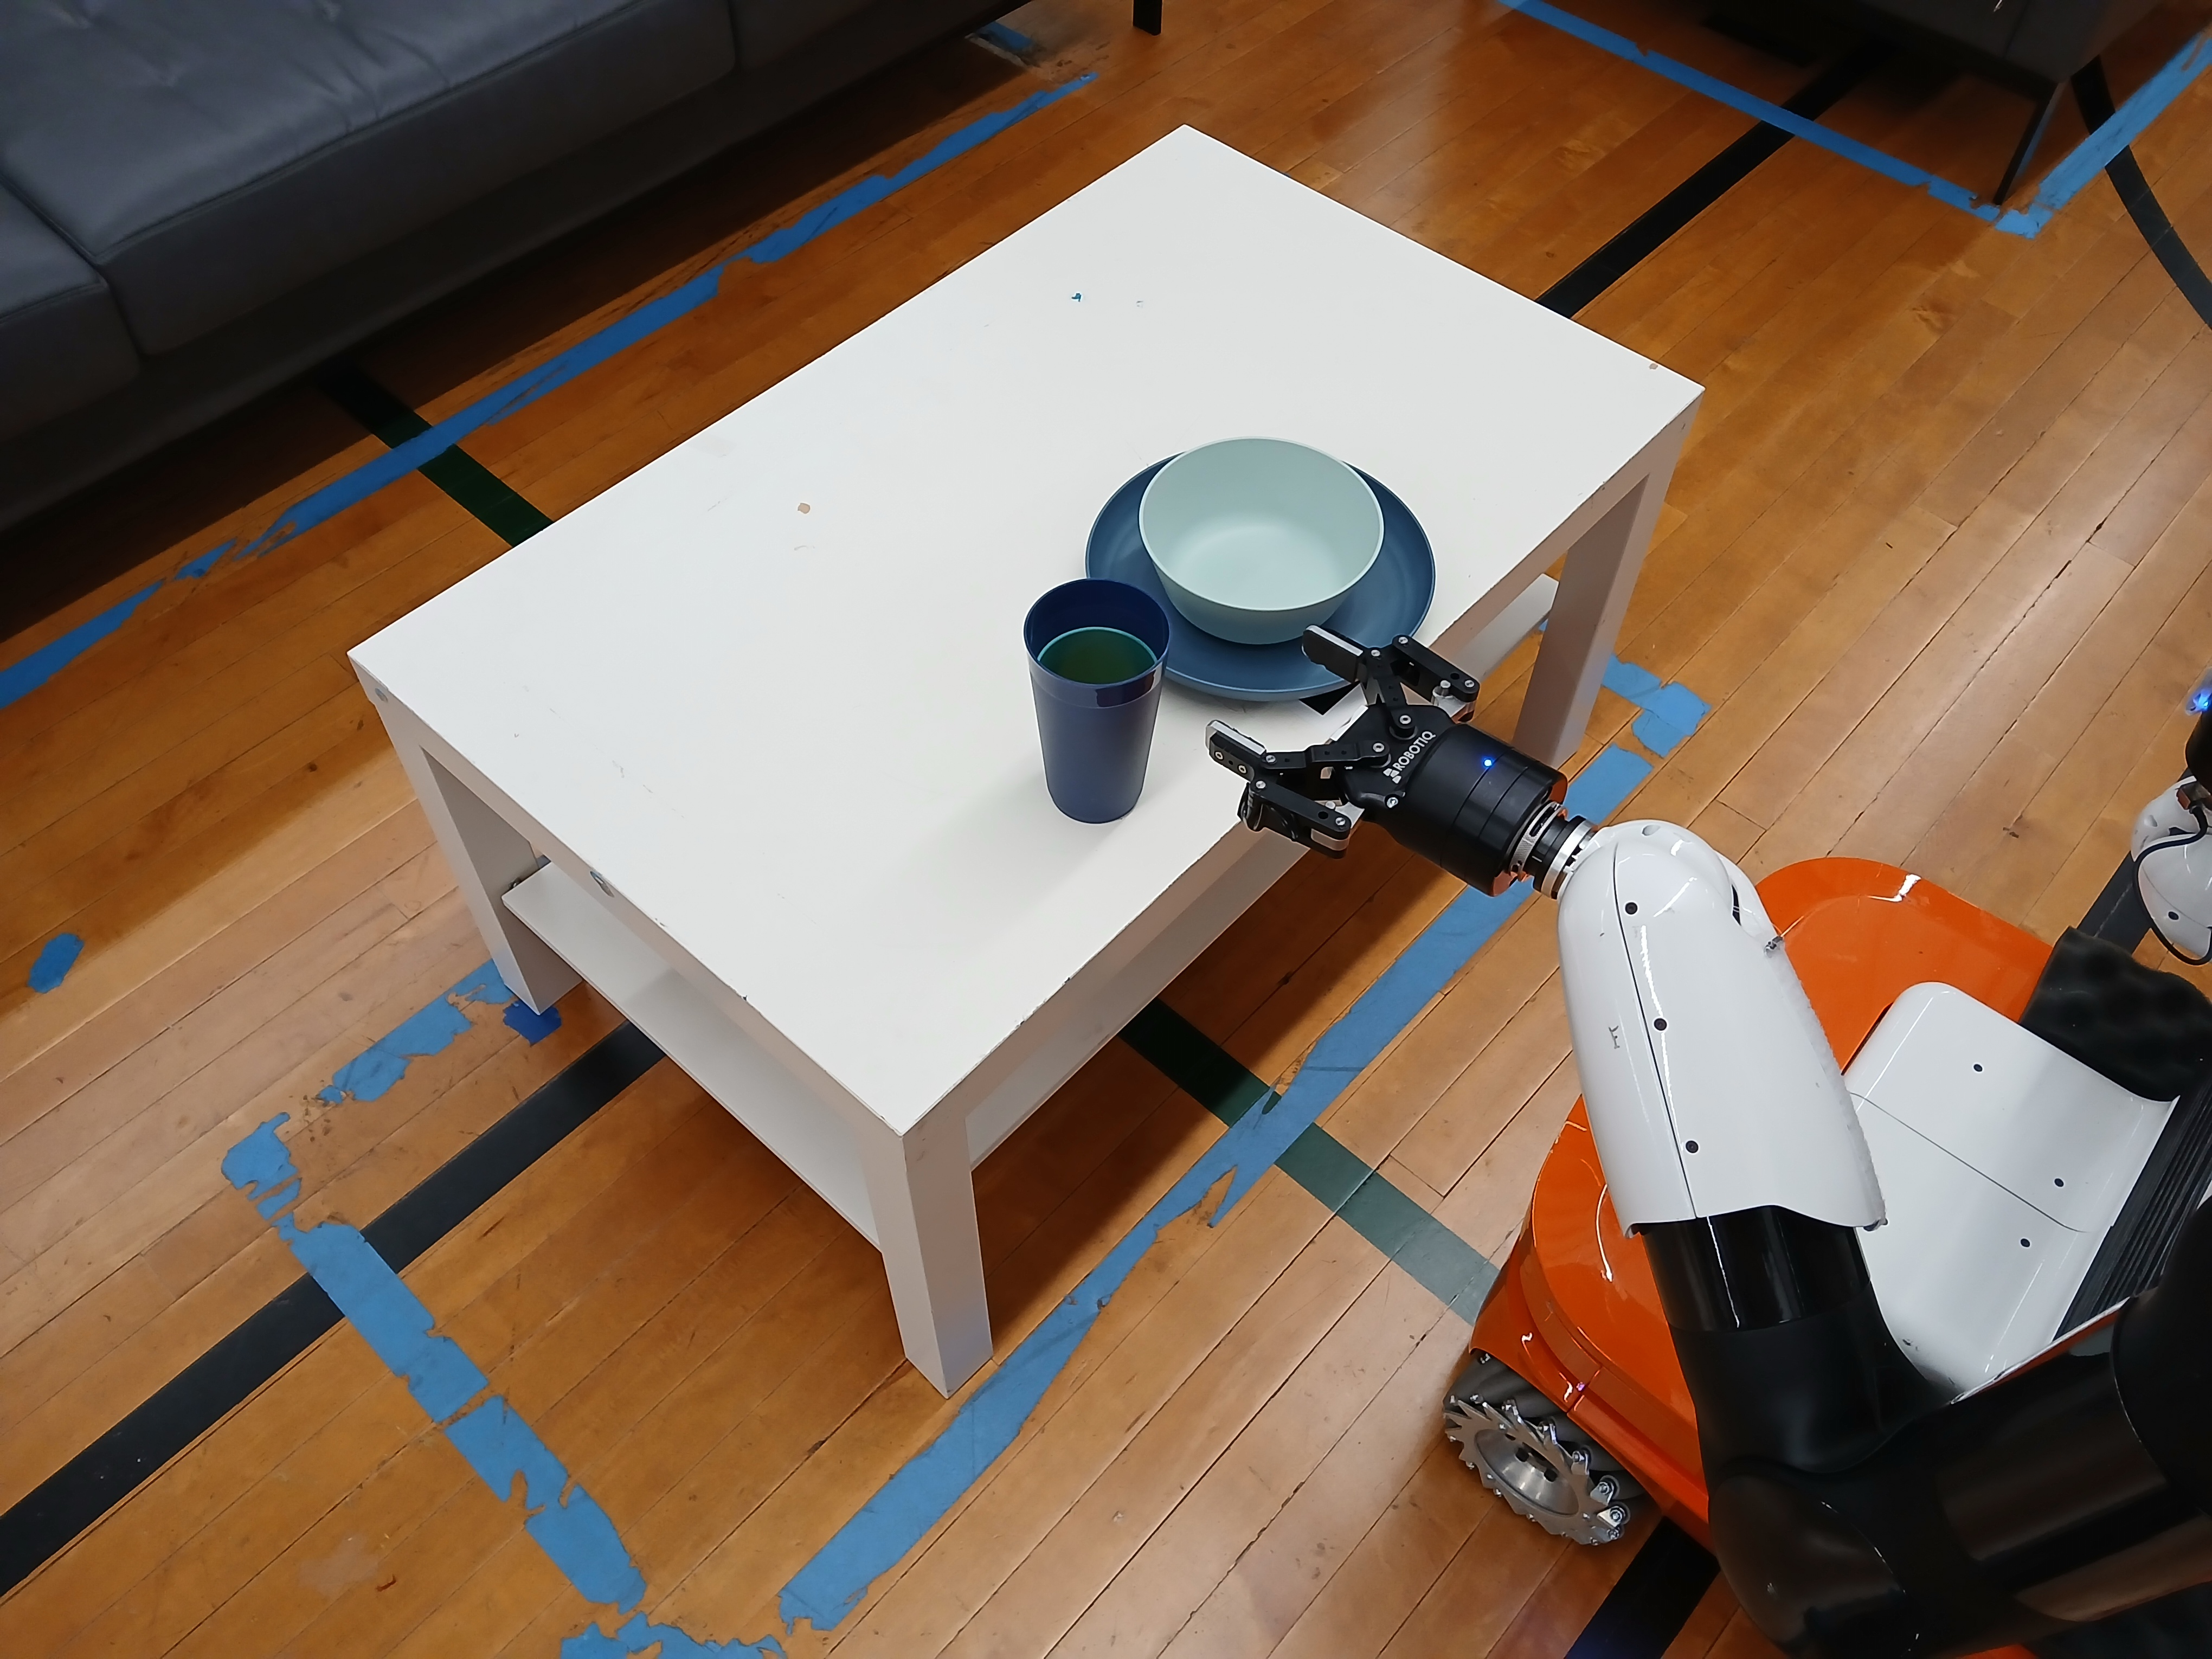
\includegraphics[width=0.32\linewidth]{figs/task_images/task1.jpg}%
\hfill%
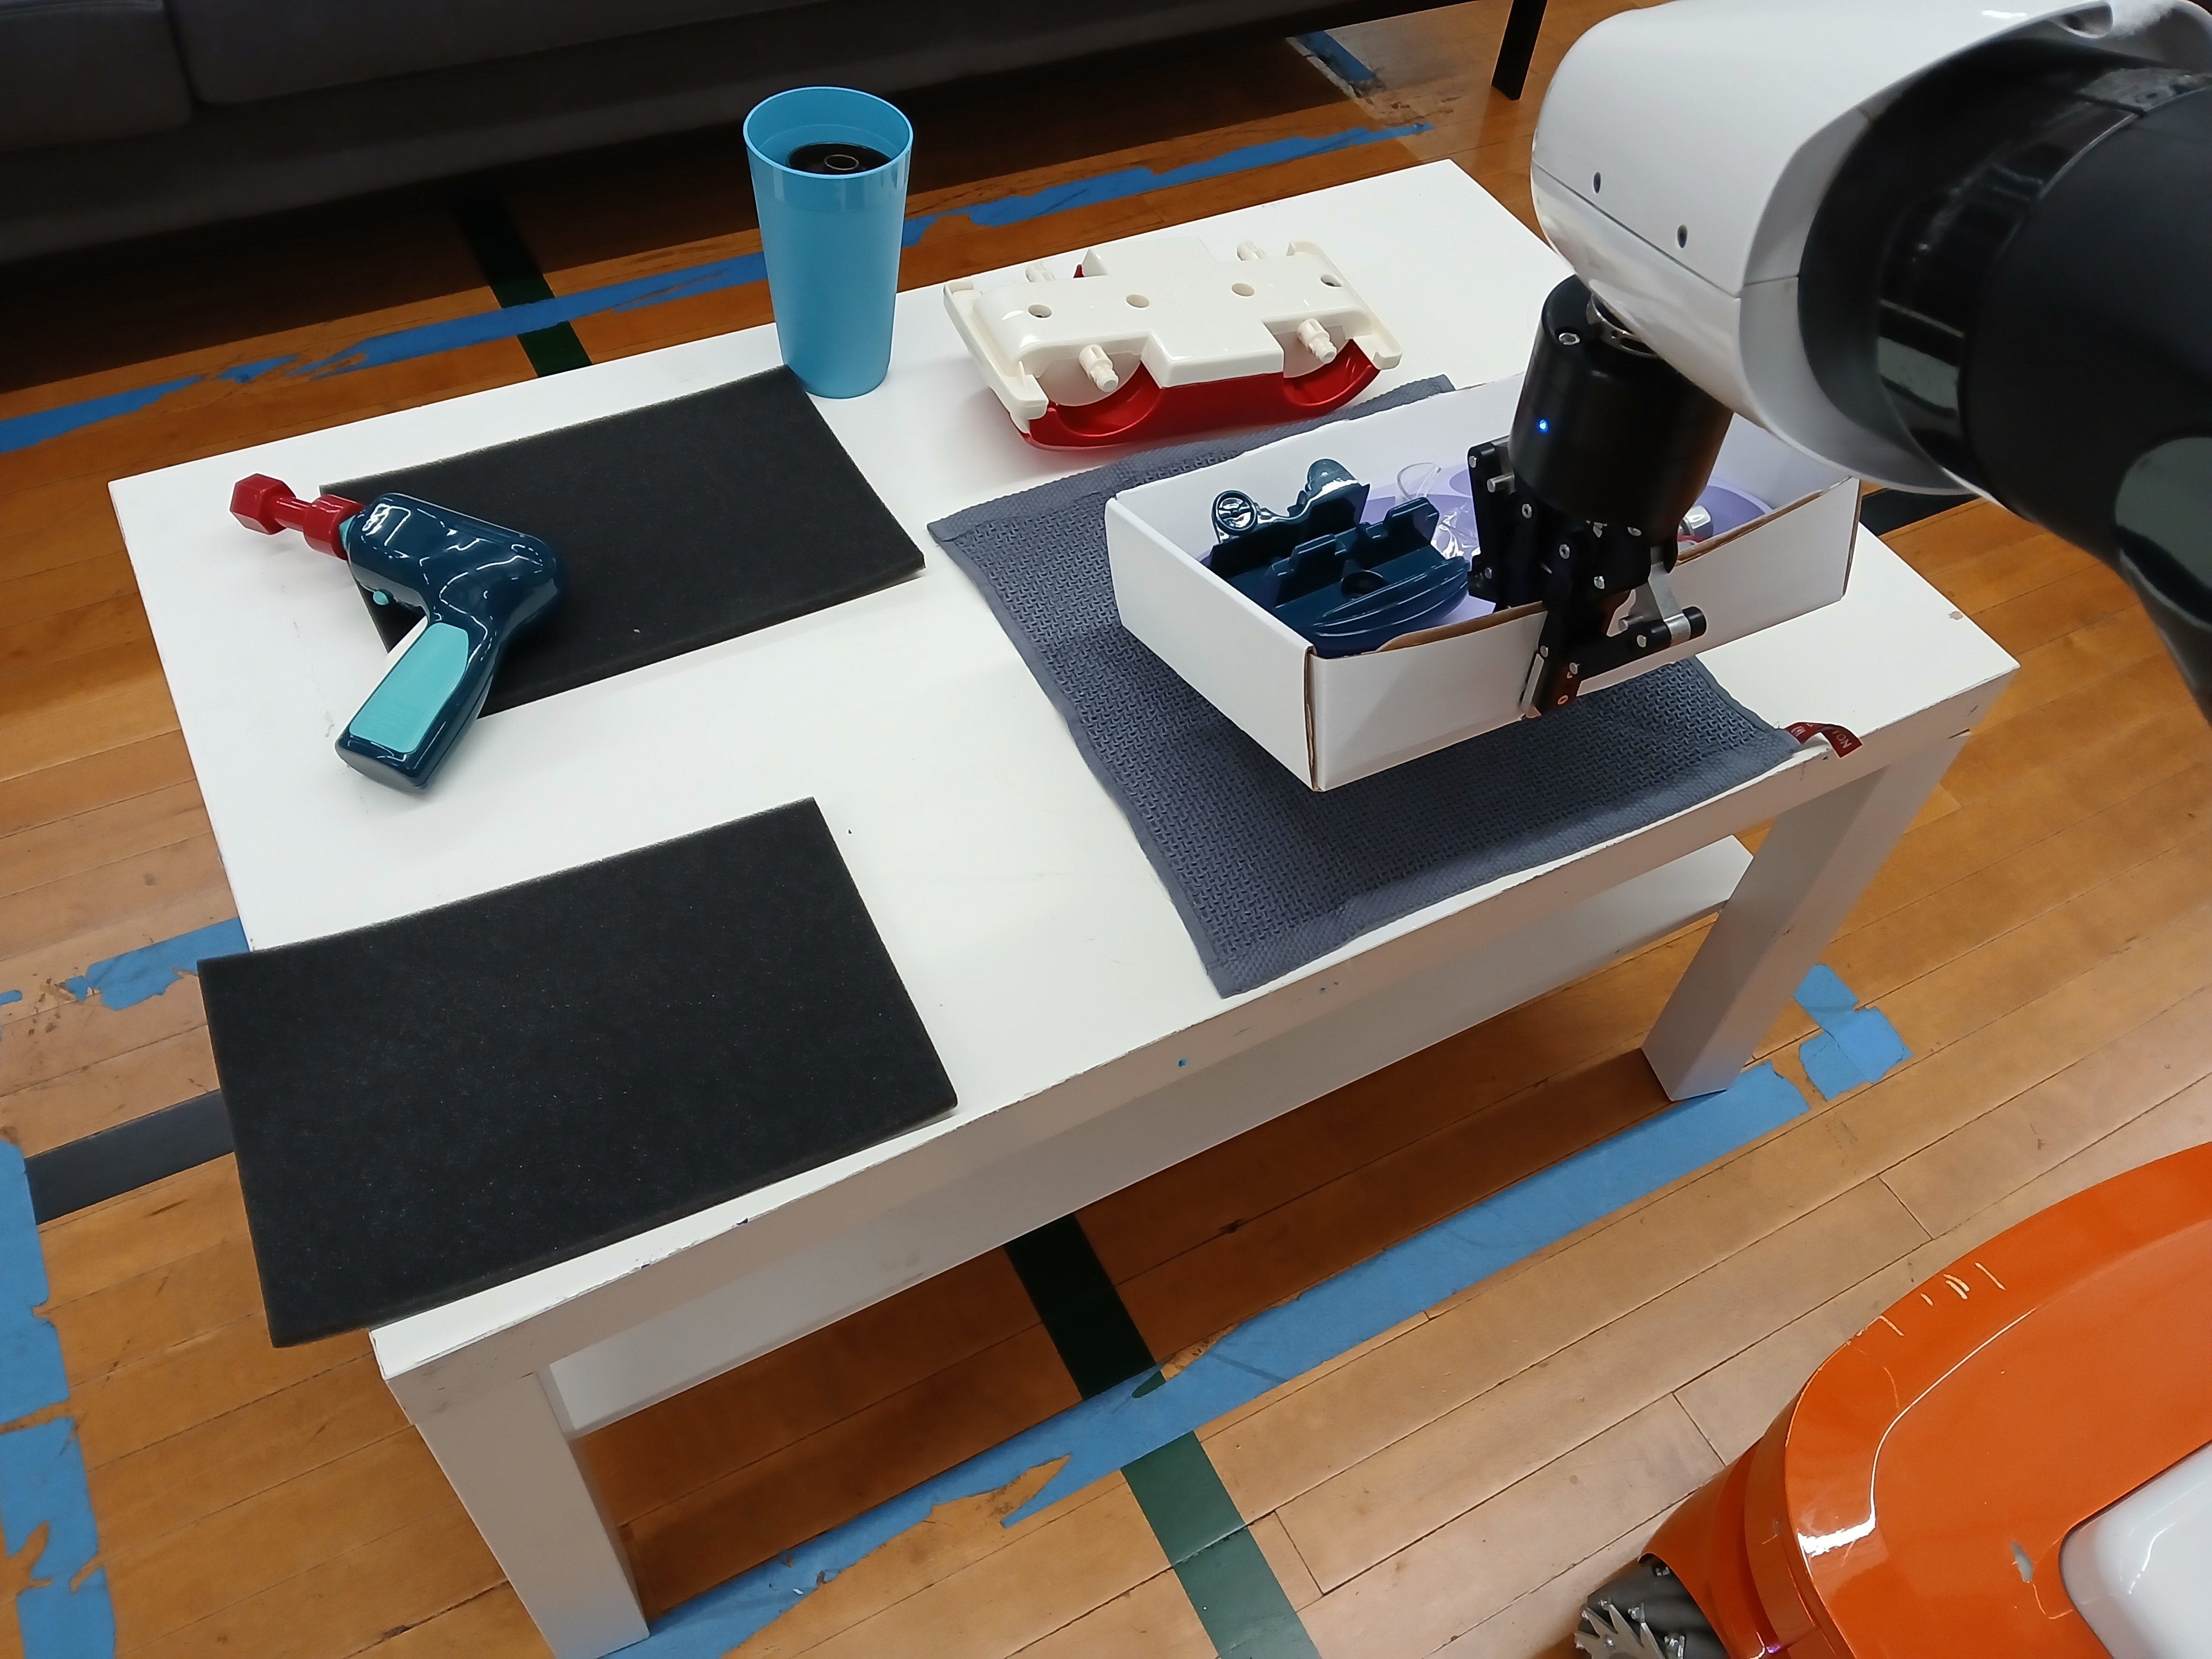
\includegraphics[width=0.32\linewidth]{figs/task_images/task2.jpg}%
\hfill%
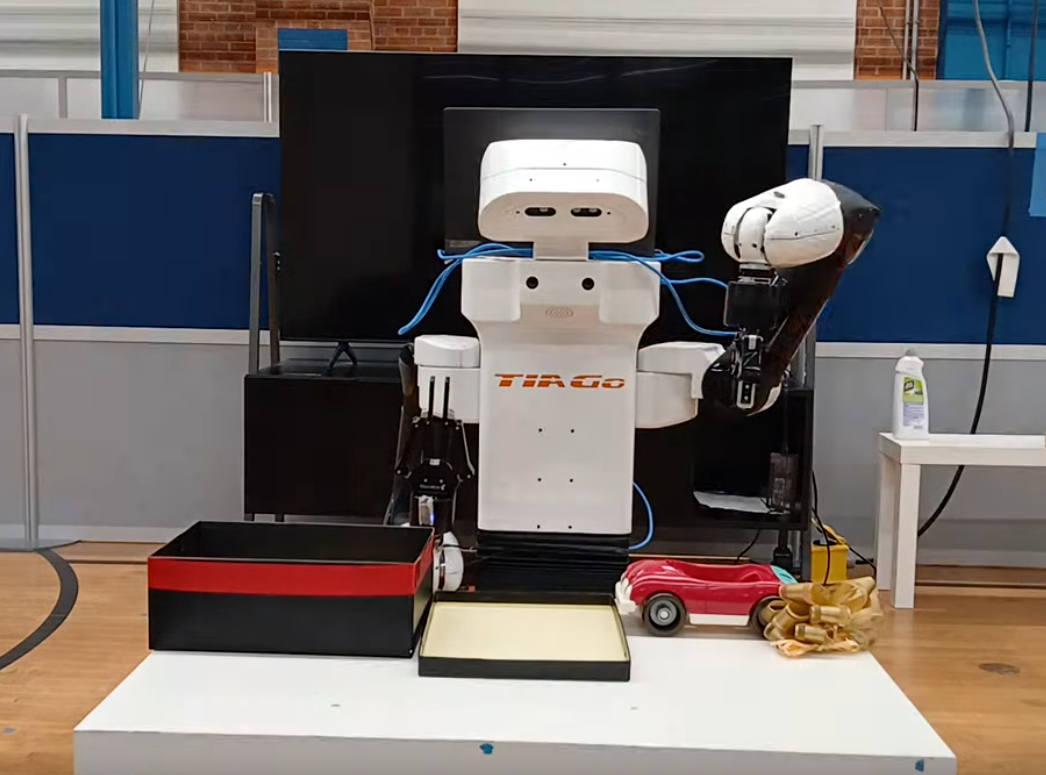
\includegraphics[width=0.32\linewidth]{figs/task_images/task3.png}\\
\caption{Real-world tasks from left to right: pouring package into bowl, assembling toy car, and packing gift box.}  
\label{fig:rw-tasks}

\end{figure}

\subsection{Real-world Task Descriptions}
\label{app:task-description}

\subsection*{Task Plans}
Our real-world tasks are depicted in Fig.~\ref{fig:rw-tasks}. In \textbf{Task 1: Pour Package into Bowl}, the plan includes (steps 1-3) bringing the package, scissors, and bowl from the kitchen to the coffee table, (step 4) opening the package with the scissors, and (step 5) pouring the opened package into the bowl. The robot is incapable of performing step 4 and must rely on human help. 
In \textbf{Task 2: Assemble Toy Car}, the plan includes (steps 1-3) bringing the parts tray, drill, and wheels from the shelf to the coffee table, (step 4) using the drill and wheel caps from the parts tray to put the wheels onto the chassis, (steps 5-6) finding and switching the drill bit, and (steps 7-8) screwing in the window and seats onto the car with the drill. The robot is incapable of performing steps 4, 6, 7, 8, and has a low success rate for step 5.
In \textbf{Task 3: Pack Gift Box}, the plan includes (step 1) folding down the gift box flap, (steps 2-3) putting the tissue paper and toy car into the box, (steps 4-6) putting on the lid, getting the ribbons from the console table, and wrapping them around the box, and (steps 7-8) cutting a piece of tape to stick the gift bow to the top of the gift box. The robot is incapable of steps 4, 6, and 7 and has a low success rate for steps 2 and 5.

The minimum human effort required to complete the tasks ranged from just one step in Task 1 to four steps in Task 2, enabling us to test how our system compares with baselines in various regimes of dependence on human collaboration.

\subsection*{Hierarchical Plan Trees for Each Task}
The robot assumes the human only knows the high-level plan. It communicates about low-level steps only when necessary, such as to split up a high-level step. These are the high and low-level step breakdowns for each task, which we call the plan hierarchy. The low-level steps are listed here in skill-parameter pair format.

Task 1: Pour Package into Bowl (5 low-level steps)
\begin{enumerate}
    \item Bring bowl and package to coffee table.
        \begin{enumerate}
            \item \texttt{pickplace(bowl, coffee\_table)}
            \item \texttt{pickplace(package, coffee\_table)}
        \end{enumerate}
    \item Open package.
        \begin{enumerate}
            \item \texttt{pickplace(scissors, coffee\_table)}
            \item \texttt{pick\_open\_place(scissors, package, coffee\_table)}
        \end{enumerate}
    \item Pour package into bowl.
        \begin{enumerate}
            \item \texttt{pick\_pour\_place(package, bowl, coffee\_table)}
        \end{enumerate}
\end{enumerate}
Task 2: Assemble Toy Car (8 low-level steps)
\begin{enumerate}
    \item Bring parts to coffee table.
        \begin{enumerate}
            \item \texttt{pickplace(parts\_tray, coffee\_table)}
            \item \texttt{pickplace(wheels, coffee\_table)}
        \end{enumerate}
    \item Assemble wheels.
        \begin{enumerate}
            \item \texttt{pickplace(drill, coffee\_table)}
            \item \texttt{put\_on(wheels, car, drill)}
        \end{enumerate}
    \item Switch drill bit.
        \begin{enumerate}
            \item \texttt{pickplace(hex\_drill\_bit, coffee\_table)}
            \item \texttt{switch(hex\_drill\_bit, drill)}
        \end{enumerate}
    \item Assemble rest of car.
        \begin{enumerate}
            \item \texttt{put\_on(window, car, drill)}
            \item \texttt{put\_on(seats, car, drill)}
        \end{enumerate}
\end{enumerate}
Task 3: Pack Gift Box (8 low-level steps)
\begin{enumerate}
    \item Assemble box.
        \begin{enumerate}
            \item \texttt{fold(box\_flap)}
        \end{enumerate}
    \item Put in gift.
        \begin{enumerate}
            \item \texttt{pickplace(gift\_tissue\_paper, box)}
            \item \texttt{pickplace(toy\_car, box)}
        \end{enumerate}
    \item Seal the box.
        \begin{enumerate}
            \item \texttt{cover(box\_lid, box)}
            \item \texttt{pickplace(ribbons, coffee\_table)}
            \item \texttt{wrap(ribbons, box)}
        \end{enumerate}
    \item Decorate the box.
        \begin{enumerate}
            \item \texttt{cut\_put(tape, scissors, box)}
            \item \texttt{pickplace(gift\_bow, box\_lid)}
        \end{enumerate}
\end{enumerate}

\subsection{Dialog Excerpts from our User Studies}
\label{app:dialog-excerpt}

\subsubsection{Convincing a Reluctant User to Perform a Step}
Our system flexibly handles long dialog interactions like the following in Task 1 (opening and pouring the package into the bowl), where it manages to convince the human to help with opening the package.

\begin{dialogue}
\speak{Robot}{Could you please open the package using the scissors on the coffee table? Thank you so much!}
\speak{Human}{There are no scissors on the coffee table.}
\speak{Robot}{Let's collaborate to open the package! I can place the scissors onto the coffee table, and you can then use them to open the package. Thank you for your help!}
\speak{Human}{I think you should bring the scissors, and then you should use the scissors to open the package.}
\speak{Robot}{I'm happy to place the scissors on the coffee table for you. However, I'm not able to open the package with the scissors and place everything on the table. Let me know if there's anything I can do to assist.}
\speak{Human}{Ok, if you bring the scissors, then I will open the package with the scissors.}
\speak{Robot}{Great! I'll happily place the scissors on the coffee table. Thank you for taking care of opening the package with the scissors!}
\speaknoquote{Robot}{[brings the scissors]}
\speak{Human}{Thanks for bringing the scissors!}
\speak{Robot}{Could you please open the package with scissors and place it on the coffee table? Thank you!}
\speak{Human}{Ok, I will do that now!}
\speaknoquote{Human}{[opens the package]}
\end{dialogue}

\subsubsection{Failure Case}
In this example, \ours{} is unable to act on human-provided motion-level feedback (making the tissue paper ``lay flatter''). Additionally, \ours{} misunderstands the human and thinks they are talking about the ribbons step when the human is still talking about the tissue paper.
\begin{dialogue}
\speak{Human}{Please pack the gift.}
\speaknoquote{Robot}{[Puts tissue paper into the box.]}
\speak{Human}{It would be nice if the parchment was laying flatter.}
\speak{Human}{The compartment is kind of squished underneath the car. If you can hold the car for me, I can fix the parchment quickly.}
\speak{Robot}{I'm sorry, but I can't cover the box with the lid. Could you help with that part? Thank you so much! Could you kindly help with sealing the box? Specifically, could you cover the box with the lid? Thank you so much for your assistance!}
\speak{Human}{Yeah, I can, but can we fix the parchment first? If you can pick up the toy car, I can fix the parchment.}
\speak{Robot}{I'm delighted to hear you'll help! Unfortunately, I won't be able to wrap the ribbons around the box.}
\speak{Human}{Okay, that's fine. We can get to that later. Let me put the lid to the box on and then we can talk about the next steps.}
\end{dialogue}

See our website for the \href{https://robin-lab.cs.utexas.edu/MicoBot/user_study_dialog.html}{complete set of dialogs and operations in our human trials}. Contrast them with the \href{https://robin-lab.cs.utexas.edu/MicoBot/baseline_dialog.html}{dialog of our user studies with the LLM baseline}, which exhibit considerably less mixed-initiative dialog and collaborative success.

\subsection{\ours{} Implementation Details}
\label{app:ours-details}
\subsection*{Robot Q-function $Q_{R}$ training in OmniGibson}

\begin{figure}[h!]
  \centering

  % Group 1: Images A and B (touching)
  \begin{subfigure}[b]{0.49\textwidth}
    \centering
    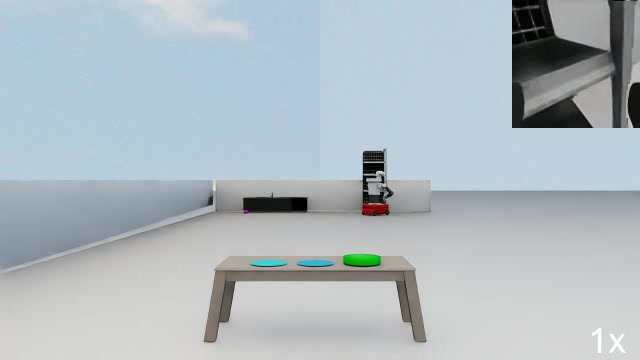
\includegraphics[width=0.495\textwidth]{figs/omnigibson_images/task1_pick_pkg.jpg}%
    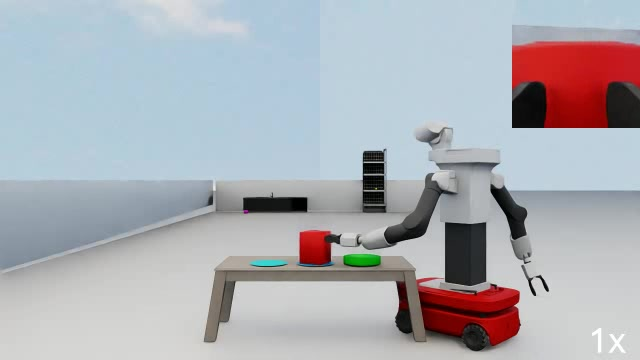
\includegraphics[width=0.495\textwidth]{figs/omnigibson_images/task1_place_pkg.jpg}
    \caption*{Task 1: Pick package from shelf (left) and place on coffee table (right).}
  \end{subfigure}
  \hfill
  % Group 2: Images C and D (touching)
  \begin{subfigure}[b]{0.49\textwidth}
    \centering
    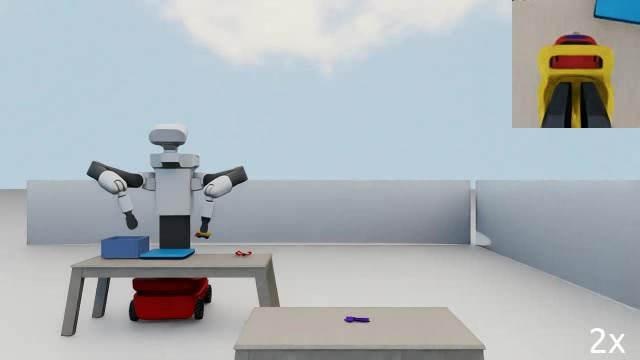
\includegraphics[width=0.495\textwidth]{figs/omnigibson_images/task3_pick_car.jpg}%
    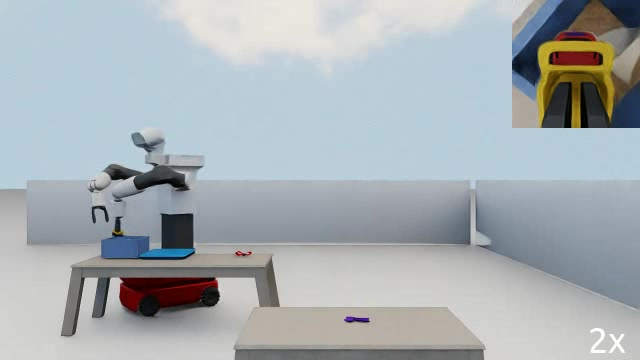
\includegraphics[width=0.495\textwidth]{figs/omnigibson_images/task3_place_car.jpg}
    \caption*{Task 3: Pick toy car from coffee table (left) and place into gift box (right).}
  \end{subfigure}

  \caption{Frames from primitive rollouts in OmniGibson for task 1 (left two images) and task 3 (right two images). Left and right images within each task are frames near the beginning and end, respectively, of each skill. The square image at the top right of each frame represents the robot's camera view observation.}
  \label{fig:omnigibson}
\end{figure}

To train Q-functions for the robot, we first create a simulated OmniGibson environment with a PAL Tiago robot and an environment that roughly matches the relative locations of the relevant furnitures and objects. We then implemented each real-world skill first in OmniGibson.
Fig.~\ref{fig:omnigibson} depicts example frames from primitives in task 1 and task 3 we ran in the OmniGibson simulator to collect sample Q-values for each skill.

We collected samples of the form $(o, a, \mathcal{T})$, where $o$ is the initial observation of the world, $a$ is the skill-parameter pair $(\omega, \theta)$ taken by the robot at $o$, and $\mathcal{T}$ is the number of timesteps the robot takes to succeed at $a$ from $o$. If the robot does not succeed in its execution, then $\mathcal{T}$ is set to some fixed constant representing the maximum number of timesteps allowed in each skill-parameter execution.

To train our Q-functions, we collect roughly 100 samples for each action $a$ and train with inputs $(o, a)$ and target Q-values $-\mathcal{T}$ using $\ell_2$ regression with the Adam Optimizer. Since our observations $o$ are primarily symbolic but include some positional information of the robot and objects, our network architecture is extremely lightweight---2 linear layers with hidden size 32 and an output size of dimension 1 for the Q-value.

\subsection*{Human Q-function $Q_{H}$ Estimation}
To estimate $Q_{H}$, we compute two terms. The first is the human's stationary cost---the number of seconds for the human to perform some task if the relevant items were all right in front of them, within grasp. This term was copied from the output of an LLM call, which was prompted with a natural language description of the low-level step in the task alongside a URL to a product description of the toy car (for task 2). The second term is the human's traveling time---the number of seconds for the human to move from their current location to the object location. This was a simple 2D euclidean distance (in meters) between the assumed human location on the couch (in the real-world user studies) and the location of the objects, divided by the average human walking speed of $1.4 m/s$. We recognize this is a crude estimate of human effort, and we discuss the limitations of this in Section~\ref{sec:limitations-future-work}.

\subsection*{Forward Dynamics Model}
Our Q-functions rely on state and action inputs. However, computing the best task allocation involves considering Q-values for future steps, which depends on having knowledge of what the future state at that step will be. This involves creating a forward dynamics model so that we can estimate the future state $n$ plan steps into the future, which can be difficult to learn accurately for continuous states. We sidestep this problem by using symbolic states for our Q-values trained in simulation and maintaining these symbolic states during our real-world experiments. A symbolic state-based forward model is feasible to hardcode in our problem setting because we assume that each action affecting change in the world is a skill-parameter physical primitive, where the effect is quite easy to specify symbolically. For instance, the effect of \texttt{pickplace(bowl, coffee\_table)} is that the bowl moves from its original furniture to the coffee table. Though this is a limitation of our method, learning a forward dynamics model is not a contribution of our work, so we leave the extension of our approach to continuous state representations to future work.

\subsection{Additional Real-world Baselines and Success Rate / Human Effort Efficiency Metrics}
\label{app:more-rw-baselines-h-effort-efficiency}

In Table~\ref{tab:more-rw-baselines-effort-efficiency}, we compute two more oracle baselines based on our existing real-world experiments that help us understand the performance of \ours{} and the LLM-baseline: (B1) LLM baseline + \textit{oracle} skills + \textit{oracle} human (100\% helpful), and (B2) \textit{Oracle} task allocator (Robot performs all steps it has $>0\%$ success rate on) + real-world skills + \textit{oracle} human. While the real-world LLM baseline achieved 27.8\% success rate (as seen in Table~\ref{tab:real-world}), (B1) achieved 33.3\%, suggesting that the \textbf{LLM baseline was slightly hindered by primitive failures.} Even with an oracle task allocation, (B2) achieves only $44\%$ success, underperforming our method at $77.8\%$, demonstrating the importance of our method optimizing for task completion while minimizing human effort.

We also compute average human effort (seconds) and success rate per second of human effort. Our method uses human effort nearly as efficiently (0.83) as the oracle baselines (B1, 0.78; B2, 1.0). While the LLM baseline performs the best along this metric at 1.19, its advantage is primarily achieved solely through successes on the first task. On the two more temporally-extended tasks, our method matches or outperforms all baselines in success rate per unit of human effort.

\begin{table}[ht!] % Note: For a two-column document, table* spans both columns. table fills one column.
\caption{Additional Real-world Baselines and Human Effort Efficiency}
\label{tab:more-rw-baselines-effort-efficiency}
\centering
\resizebox{\columnwidth}{!}{ % Use \columnwidth if the table should fit within a single column
\begin{tabular}{rlcccc}
\toprule
\textbf{Real-World Task} &
\textbf{Metric} &
\textbf{LLM baseline} &
\textbf{\ours{}} &
% \multicolumn{1}{c}{\begin{tabular}{@{}c@{}}\textbf{LLM baseline} \\ \textbf{+ oracle skills} \\ \textbf{+ oracle human}\end{tabular}} &
% \multicolumn{1}{c}{\begin{tabular}{@{}c@{}}\textbf{Oracle task allocator} \\ \textbf{+ real-world skill} \\ \textbf{+ oracle human}\end{tabular}} \\
\textbf{(B1)} &
\textbf{(B2)} \\
\midrule
\multirow{4}{*}{\textbf{Pour Package in Bowl}} & Success Rate (\%, $\uparrow$) & 83 & \textbf{100} & 83 & 41 \\
& Steps Completed (\%, $\uparrow$) & 93.3 & \textbf{100} & 93.3 & 64.5 \\
% & Human Effort (\% steps completed) & 5 & 21 & 25 & 20 \\
& Human Effort (seconds) & 36.7 & 48 & 46.7 & 32.7 \\
& Success Rate (\%) / Human Effort (s) ($\uparrow$) & \textbf{2.3} & 2.1 & 1.8 & 1.3 \\
\midrule
\multirow{4}{*}{\textbf{Assemble Toy Car}} & Success Rate (\%, $\uparrow$) & 0 & \textbf{67} & 0 & 11 \\
& Steps Completed (\%, $\uparrow$) & 29 & \textbf{94} & 54.2 & 43.2 \\
% & Human Effort (\% steps completed) & 5 & 60 & 23.1 & 50 \\
& Human Effort (seconds) & 20.8 & 197.3 & 56.7 & 55.0 \\
& Success Rate (\%) / Human Effort (s) ($\uparrow$) & 0 & \textbf{0.3} & 0 & 0.2 \\
\midrule
\multirow{4}{*}{\textbf{Pack Gift Box}} & Success Rate (\%, $\uparrow$) & 0 & 67 & 17 & \textbf{80} \\
& Steps Completed (\%, $\uparrow$) & 50 & 88 & 62.5 & \textbf{97.5} \\
% & Human Effort (\% steps completed) & 21 & 35 & 33.3 & 37.5 \\
& Human Effort (seconds) & 12.5 & 37.5 & 25 & 45.0 \\
& Success Rate (\%) / Human Effort (s) ($\uparrow$) & 0 & \textbf{1.8} & 0.68 & \textbf{1.8} \\
\midrule
\multirow{4}{*}{\textbf{Average}} & Success Rate (\%, $\uparrow$) & 27.8 & \textbf{77.8} & 33.3 & 44.0 \\
& Steps Completed (\%, $\uparrow$) & 58.2 & \textbf{93.8} & 70 & 68.4 \\
% & Human Effort (\% steps completed) & 10.4 & 38.8 & 27.1 & 35.8 \\
& Human Effort (seconds) & 23.3 & 94.3 & 42.8 & 44.2 \\
& Success Rate (\%) / Human Effort (s) ($\uparrow$) & \textbf{1.19} & 0.83 & 0.78 & 1.00 \\
\bottomrule
\end{tabular}
} % End of \resizebox
\vspace{-1em}
% \caption{Comparison of different system configurations across three real-world tasks and their average performance for key metrics.}
\label{tab:new-results}
\end{table}

\subsection{Statistical Testing}
In Table~\ref{tab:stat-tests}, we perform statistical tests on our user study results from Table~\ref{tab:real-world}. All results are statistically significant ($p$-val. column).
% See also the MicoBot vs. LLM baseline \href{https://mico-bot.github.io/static/images/likert_plot.png}{Likert score distribution}.

\begin{table}[ht!]
\caption{Statistical Testing on Results Shown in Table~\ref{tab:real-world}}
\label{tab:stat-tests}
\centering
\resizebox{\columnwidth}{!}{
\begin{tabular}{lccccc}
\toprule
\textbf{Metric} &
\textbf{\ours{} (ours)} &
\textbf{LLM baseline} &
\textbf{Statistical Test} &
\textbf{Test statistic} &
\textbf{$p$-val.} \\
\midrule
Overall User Satisfaction ($\uparrow$, /5) & $3.61 \pm 0.95$ & $2.5 \pm 1.38$ & \multirow{4}{*}{\begin{minipage}{2cm}
    Wilcoxon \\ Signed-Rank
  \end{minipage}} & $W=17.0$ & $0.023540$ \\
Communicative Ability ($\uparrow$, /5) & $3.72 \pm 1.41$ & $2.33 \pm 1.56$ & & $W=8.5$ & $0.009233$ \\
Asked for Suitable Amt. of Help ($\uparrow$, /5) & $3.61 \pm 0.83$ & $2.56 \pm 1.42$ & & $W=15.0$ & $0.008636$ \\
Awareness of Its Limitations ($\uparrow$, /5) & $3.94 \pm 0.85$ & $2.61 \pm 1.53$ & & $W=16.0$ & $0.006502$ \\
\midrule
Success Rate (\%, $\uparrow$) & $77.8 \pm 15.7$ & $27.8 \pm 39.3$ & Fisher's Exact & -- & $0.006709$ \\
\midrule
Steps Completed (\%, $\uparrow$) & $93.8 \pm 15.2$ & $57.5 \pm 30.6$ & Wilcoxon Signed-Rank & $W=0.0$ & $0.002031$ \\
\bottomrule
\end{tabular}
} % End of \resizebox
% \caption{Key statistical performance metrics of ours vs. baseline.}
\label{tab:performance_comparison}
\end{table}

\subsection{Mixed-Initiative Dialog: Real-world Metrics}
\label{app:mixed-init-dialog-metrics}

\begin{table}[h]
\caption{Mixed-Initiative Dialog Metrics}
\label{tab:mixed-init-dialog-metrics}
\centering
\resizebox{\columnwidth}{!}{
\begin{tabular}{lcc}
\toprule
\begin{tabular}{@{}c@{}}\textbf{Metric (avg over each trial)} \\ R = Robot, H = human \end{tabular} &
\textbf{\ours{} (ours)} &
\textbf{LLM baseline} \\
\midrule
\# R-Helpreqs & $2.9 \pm 1.4$ & $0.9 \pm 1.1$ \\
Initial H acceptance rate & $55\% \pm 35\%$ & $70\% \pm 46\%$ \\
H acceptance rate after R-negotiation & $86\% \pm 27\%$ & $75\% \pm 40\%$ \\
R-init dialogs & $3.6 \pm 1.8$ & $0.9\pm 1.1$ \\
H-init dialogs & $2.9 \pm 2.4$ & $2.3 \pm 2.9$ \\
Initiative Shifts & $2.4 \pm 2.1$ & $1.1 \pm 1.6$ \\
\bottomrule
\end{tabular}
} % End of \resizebox
% \caption{Dialog statistics.}
\label{tab:dialog_stats}
\end{table}

We evaluate the dialog of all our real-world user studies across the three tasks and compile mixed-initiative metrics of \ours{} and the baseline in Table~\ref{tab:dialog_stats}.
\textbf{\ours{} boosts human acceptance of help requests from $\mathbf{55\%}$ to $\mathbf{86\%}$ with negotiation.} However, the LLM baseline, which succeeded at a far lower rate in our user studies, made far fewer requests (0.9 vs. \ours{}'s 2.9) and achieves a smaller acceptance increase ($70\%$ to $75\%$). \textbf{\ours{} collaborates with a high level of robot and human initiated dialog ($\mathbf{3.6}$ robot dialog initiations vs. $\mathbf{2.9}$ human initiations, with $\mathbf{2.4}$ dialog initiative shifts/trial}), whereas the LLM trials are human-initiative driven ($0.9$ robot dialog initiations vs. $2.3$ humaan initiations, with $0.9$ initiative shifts). This suggests that mixed-initiative dialog helps enable \ours{} to have better task success outcomes and user satisfaction ratings than the LLM baseline.

\subsection{Detailed Simulation Results}
\label{app:ours-sim-results}
\subsubsection{Setup}
In simulation, we ran our method, the three baselines (RL, LLM, random), and our method's four ablations (no $p_{H, t}$ estimation, no plan hierarchy, no R-initiative dialog, and no H-initiative dialog) on eight different settings of parameterized humans in simulation. These eight settings were a cross product of 2 dialog mood settings (positive and negative) and 4 ground-truth $\tilde{p}_{H, t} \in \{0.0, 0.3, 0.7, 1.0\}$ settings (following the notation introduced in Appendix~\ref{app:extra-exps}, where the $\tilde{p}$ denotes the ground truth probability while the plain $p$ denotes our estimate). $10$ trials were run for each method in each of the eight settings for the parameterized human.

\subsubsection{Simulation Experiments}

In Table~\ref{tab:sim-results}, we show the results of our method in a simulation version of our real-world Task 1. Our method performs better than baselines especially in scenarios where $\tilde{p}_{H, t}$ is low, because our method is able to take initiative through dialog, such as by proposing ways to split up steps to make them more achievable with the simulated human. The averages in Table~\ref{tab:sim-results} are plotted in Fig.~\ref{fig:rw-success-vs-human-effort}.

\begin{table*}[h]
\centering
\caption{Simulation Task 1 Performance across different $\tilde{p}_{H, t}$ Values and Language Sentiments.}
\label{tab:sim-results}
\resizebox{\textwidth}{!}{
\begin{tabular}{|l|l|c|c|c|c|c|c|c|c|c|}
\cline{3-10}
\multicolumn{2}{c|}{} & \multicolumn{8}{c|}{\textbf{Human Parameters (Mood, $\tilde{p}_{H, t}$)}} & \multicolumn{1}{c}{} \\
\hline
\multirow{2}{*}{\textbf{Method}} & \multirow{2}{*}{\textbf{Metric}} 
& \multicolumn{4}{c|}{\textbf{Positive Mood}} 
& \multicolumn{4}{c|}{\textbf{Negative Mood}} 
& \multirow{2}{*}{\textbf{Avg. (\%)}} \\
\cline{3-10}
 &  & \textbf{0.0} & \textbf{0.3} & \textbf{0.7} & \textbf{1.0} 
 & \textbf{0.0} & \textbf{0.3} & \textbf{0.7} & \textbf{1.0} & \\
\hline
\multirow{3}{*}{\textbf{Ours}} 
& Success Rate & 3/10 & 6/10 & 9/10 & 10/10 & 1/10 & 4/10 & 9/10 & 9/10 & \textbf{63.75} \\
& Num Plan Steps Completed & 3.6/5 & 4.2/5 & 4.8/5 & 5.0/5 & 3.2/5 & 3.8/5 & 4.8/5 & 4.5/5 & \textbf{84.5} \\
& Prop. Plan Steps done by Human & 0.1667 & 0.2381 & 0.3125 & 0.4 & 0.03125 & 0.1579 & 0.354 & 0.377 & 25.47 \\
\hline
\multirow{3}{*}{\textbf{LLM Baseline}} 
& Success Rate & 2/10 & 2/10 & 4/10 & 7/10 & 3/10 & 6/10 & 6/10 & 6/10 & 45 \\
& Num Plan Steps Completed & 3.4/5 & 3.4/5 & 3.7/5 & 4.4/5 & 3.6/5 & 4.2/5 & 4.0/5 & 4.2/5 & 77.25 \\
& Prop. Plan Steps done by Human & 0.0588 & 0.05882 & 0.2162 & 0.1591 & 0.1111 & 0.1428 & 0.175 & 0.166 & 13.6 \\
\hline
\multirow{3}{*}{\textbf{Random Agent}} 
& Success Rate & 2/10 & 5/10 & 6/10 & 7/10 & 2/10 & 3/10 & 6/10 & 7/10 & 47.5 \\
& Num Plan Steps Completed & 3.4/5 & 3.5/5 & 4.0/5 & 4.4/5 & 3.4/5 & 2.8/5 & 4.0/5 & 4.4/5 & 74.75 \\
& Prop. Plan Steps done by Human & 0.1176 & 0.4286 & 0.525 & 0.7045 & 0.1176 & 0.2143 & 0.525 & 0.7045 & 41.71 \\
\hline
\multirow{3}{*}{\textbf{RL}} 
& Success Rate &  0/10 & 1/10 & 4/10 & 10/10 & 0/10 & 1/10 & 4/10 & 10/10 & 37.5 \\
& Num Plan Steps Completed & 2.4/5 & 2.3/5 & 3.4/5 & 5.0/5 & 2.4/5 & 2.3/5 & 3.4/5 & 5.0/5 & 65.5 \\
& Prop. Plan Steps done by Human & 0.125 & 0.1739 & 0.4412 & 0.54 & 0.125 & 0.1739 & 0.4412 & 0.54 & 32.0 \\
\hline
\multirow{3}{*}{\textbf{Only R Init}} 
& Success Rate & 0/10 & 3/10 & 9/10 & 10/10 & 0/10 & 5/10 & 9/10 & 10/10 & 57.5 \\
& Num Plan Steps Completed & 3.0/5 & 3.6/5 & 4.8/5 & 5.0/5 & 3.0/5 & 4.0/5 & 4.8/5 & 5.0/5 & 83 \\
& Prop. Plan Steps done by Human & 0.0 & 0.1111 & 0.3542 & 0.4 & 0.0 & 0.225 & 0.354 & 0.4 & 23.05 \\
\hline
\multirow{3}{*}{\textbf{Only H Init}} 
& Success Rate & 0/10 & 0/10 & 0/10 & 0/10 & 2/10 & 0/10 & 0/10 & 2/10 & 5.0 \\
& Num Plan Steps Completed & 3.0/5 & 3.0/5 & 3.0/5 & 3.0/5 & 3.2/5 & 3.0/5 & 3.0/5 & 3.3/5 & 61.25 \\
& Prop. Plan Steps done by Human & 0.0 & 0.0 & 0.0 & 0.0/3.0 & 0.1875 & 0.0 & 0.0 & 0.1212 & 3.86 \\
\hline
\multirow{3}{*}{\textbf{Ours w/o p\_help}} 
& Success Rate & 3/10 & 5/10 & 9/10 & 10/10 & 2/10 & 3/10 & 9/10 & 9/10 & 62.5 \\
& Num Plan Steps Completed & 3.6/5 & 4.0/5 & 4.8/5 & 5.0/5 & 3.4/5 & 3.4/5 & 4.8/5 & 4.7/5 & 84.25 \\
& Prop. Plan Steps done by Human & 0.1667 & 0.3 & 0.3333 & 0.38 & 0.1176 & 0.2059 & 0.3125 & 0.4468 & 28.29 \\
\hline
\multirow{3}{*}{\textbf{Ours w/o Plan Hier.}} 
& Success Rate & 2/10 & 4/10 & 7/10 & 10/10 & 0/10 & 3/10 & 4/10 & 8/10 & 47.5 \\
& Num Plan Steps Completed & 3.4/5 & 3.8/5 & 4.0/5 & 5.0/5 & 3.0/5 & 3.4/5 & 3.6/5 & 4.2/5 & 76 \\
& Prop. Plan Steps done by Human & 0.0588 & 0.1316 & 0.25 & 0.24 & 0.0667 & 0.1176 & 0.1944 & 0.2381 & 16.22 \\
\hline
\end{tabular}
}
\end{table*}

\subsection{User Study Details}
\label{app:user-study-details}
\subsubsection{User Instructions}
Users were read the following instructions at the beginning of the study. (Instructions here are shown for Task 2.)

\begin{enumerate}
    \item Thank you so much for coming for our user study! We wanted to remind you to review the RIS before proceeding, and that you may voluntarily opt-out of the study at any time.
    \item You are working with the robot to perform the task of assembling the toy car. You must use the hexagonal drill bit to screw in the wheels, and the phillips drill bit to screw in the seat and the window. [Demonstrate these steps to the human]. You and the robot operate on a shared understanding of the plan. [Read the 4 high-level steps of the plan tree for this task. Do NOT discuss the low-level steps of the plan tree.]
    \item Our goal is to simulate a home robot setting, where the human (you) is relatively busy with your own tasks, and once in a while you provide physical assistance and talk to the robot. So you are free to do work during each trial.
    \item Once the robot asks you to do a step, and you accept, you must finish that step successfully.
    \item We will perform 2 trials, each of a different method.
    \item Both you and the robot can do a subset of the steps in the plan. You will communicate with the robot to determine who does what steps.
    \item These are the objects you will work with during the task. I will move them now to their initial positions where they will start at the beginning of each trial. [Move objects to initial positions.]
    \item For safety, I will gate-keep each of the robot’s physical actions. In other words, the actions are generated by the robot itself, but they will be displayed on the laptop screen with a confirmation message, and I can either allow that physical action to be executed by the robot, or block the action from being executed if it brings the robot to an unsafe location.
    \item The robot will stay on the TV side of the coffee table, while you will sit on the couch and stay on the couch side of the coffee table.
    \item You are free to get up off the couch if you want to volunteer to perform steps that involve going to the sink or shelf, but you can only go when the robot is stationary and waiting on the other side of the coffee table. Steps are done in sequential order; our system doesn’t support parallelization (agents working simultaneously).
    \item You will be communicating to the robot through this headset. We will perform a mic-check now to make sure it can pick up your voice. [Do mic check.]
    \item Now, this is what the robot will sound like when it talkes to you. [Play audio sample of the robot.] Try responding to it, and I will see if it can hear you.
    \item The systems today can handle different kinds of dialog. (1) refusal/acceptance, (2) task allocation, such as (``Could you pour the package in the plate later?'' Or: ``I can pour the package onto the plate later.''), (3) silence---you don't need to respond to the robot every time, and (4) a proposal to split up adjacent steps, such as ``Please bring me the drill so that I can put on the wheels.'' You may engage in any of these types of dialog, and the robot may also engage in them when communicating to you.
    \item Do you have any questions before we start? I will let you know when each trial begins and ends. Sometimes trials may end prematurely.
\end{enumerate}

\subsubsection{Success Rate}
Success at each step is measured by whether the goal state of a primitive has been achieved. For instance, a \texttt{pickplace(obj, furniture)} step in the plan is marked as successfully completed if the \texttt{obj} ends up on the \texttt{furniture} after execution. This means that primitive errors (such as a pickplace operation that accidentally moves the object off of the furniture as the arm is retracting) count as a failed execution. In Table~\ref{tab:real-world}, ``\% of task steps completed'' is evaluated by tallying up all of the steps in the low-level plan that have succeeded and dividing this by the length of the plan. ``Entire Task Success Rate'' is defined as whether all plan steps in a run have been successfully completed.

\subsection{Real-world Failure Analysis}
See the failure breakdowns in our real-world trials for \ours{} (Figure~\ref{fig:ours-failure-flow-diagram}) and the LLM baseline (Figure~\ref{fig:llm-baseline-failure-flow-diagram}).

\begin{figure}[ht!]
    \centering
    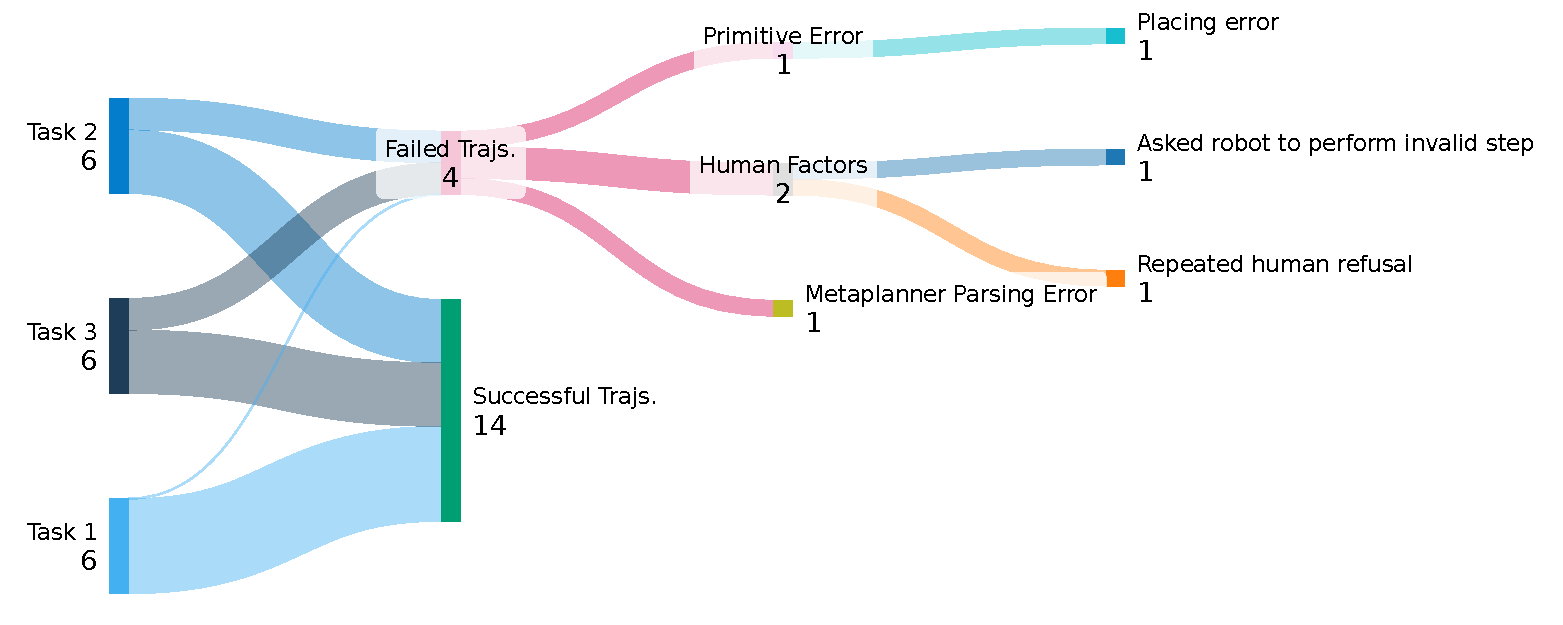
\includegraphics[width=1\columnwidth]{figs/plots/ours_failure_modes.pdf}
    \caption{\ours{} mainly fails from an inability to solicit human help. Metaplanner and primitive errors were also encountered.}
    \label{fig:ours-failure-flow-diagram}
\end{figure}

\begin{enumerate}
    \item Task 1: Cut and Pour Package into Bowl. 0 failed trials out of 6.
    \item Task 2: Assemble Toy Car. 2 failed trials out of 6. 1 failure that was rectified by human.
        \begin{itemize}
            \item 1 dialog error: user wanted robot to perform a non-step plan outside of its capabilities, and refused when robot said it wasn't able to perform it
            \item 1 primitive error: robot did not release its grasp of the drill.
            \item 1 metaplanner dialog parsing error
        \end{itemize}
    \item Task 3: Pack Gift Box. 2 failed trials out of 6.
        \begin{itemize}
            \item 1 primitive error: placed bow on box but bow dropped to floor as gripper retracted
            \item 1 termination condition triggered: human rejected robot's help request and subsequent proposals twice in a row.
        \end{itemize}
\end{enumerate}

\begin{figure}[ht!]
    \centering
    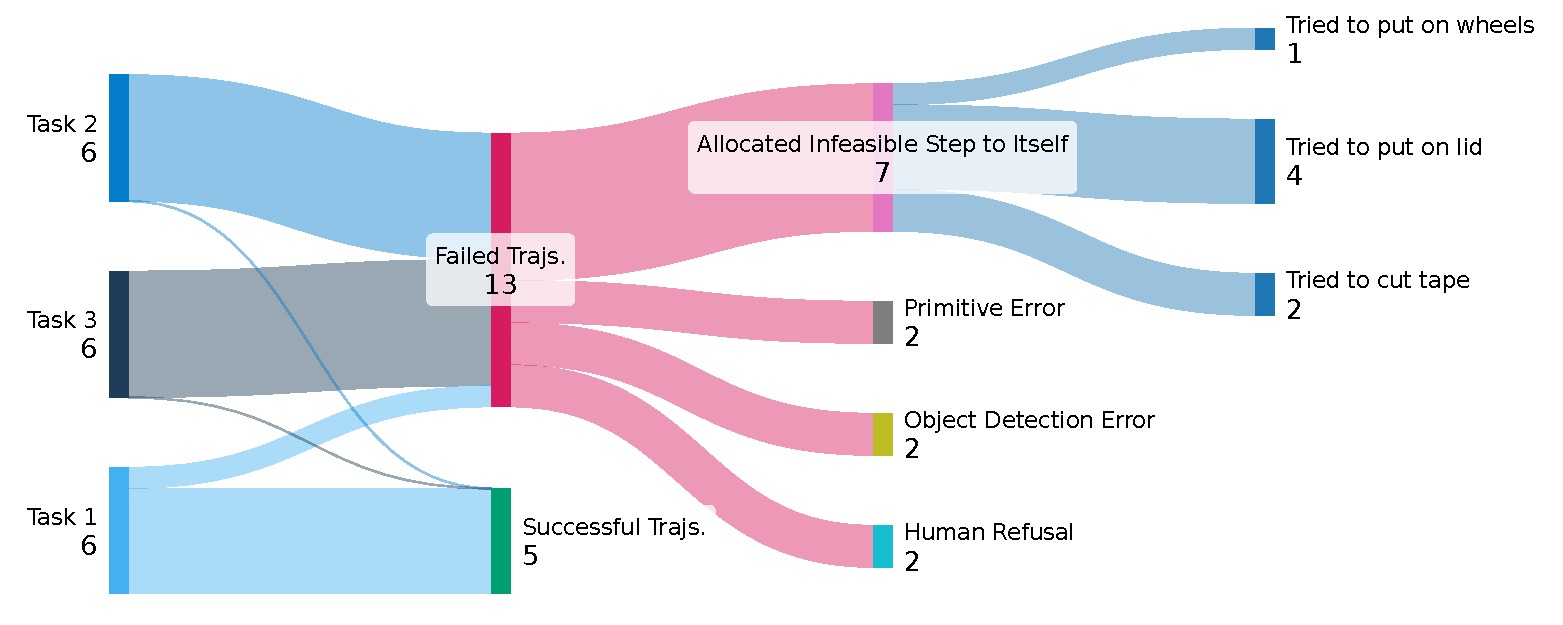
\includegraphics[width=1\columnwidth]{figs/plots/llm_failure_modes.pdf}
    \caption{The LLM baseline failed mainly by allocating itself steps it could not perform, due to the LLM's lack of knowledge of its own affordances.}
    \label{fig:llm-baseline-failure-flow-diagram}
\end{figure}

\begin{enumerate}
    \item Task 1: Cut and Pour Package into Bowl. 1 failed trials out of 6.
        \begin{itemize}
            \item 1 termination condition triggered: human rejected robot's help request twice in a row.
        \end{itemize}
    \item Task 2: Assemble Toy Car. 6 failed trials out of 6.
        \begin{itemize}
            \item 2 primitive errors: Placed the drill, but then it fell off of the table.
            \item 2 perception errors: Unable to visually find the correct location to place the object.
            \item 1 task allocation error: Allocated to put on the car wheels itself.
            \item 1 termination condition triggered: Fell into a conversational loop with the user.
        \end{itemize}
    \item Task 3: Pack Gift Box. 6 failed trials out of 6. 1 failure was rectified by human.
        \begin{itemize}
            \item 6 task allocation errors: Tried to put on the lid itself four times; tried to cut a piece of tape itself twice.
            \item 1 primitive error: Inadvertently dropped the car onto the floor as it was trying to place it.
        \end{itemize}
\end{enumerate}

\subsection{Fault Recovery}
\label{app:fault-recovery}
The metaplanner ocassionally produces faulty, non-executable code. For fault recovery, the metaplanner is automatically re-queried up to 2 additional times to create code. If these attempts also produce non-executable code, the most recent dialog from the human is ignored for 2 further, automated metaplanner requeries. These re-queries are handled by a try-except block in the iterative planner module of \ours{}.

\subsection{RL Baseline Details}
\label{app:rl-baseline}
For our RL baseline which was evaluated in simulation, we train a hierarchical policy where the high-level policy was a task allocator that outputted logits over two classes: 0 (Robot would perform current step), or 1 (Human would perform current step). If the logit for 0 is higher, then the image observation is passed into the low-level robot policy that decides the discrete physical action to take in the world. Otherwise, the robot asks the human through a verbal action for help on that step. We use sparse rewards, issued only when all 5 steps were completed in the task, in the proper order.

We initially trained the RL policy on two simulated human settings: one where the human ground truth $\tilde{p}_{H, t} = 1.0$, and another where $\tilde{p}_{H, t} \sim U[0, 1]$. We were unable to obtain policies with any non-zero training returns after thousands of iterations on the latter setting, so we only report results on the former setting, which explains why the RL policy does not perform well when $\tilde{p}_{H, t}$ is low.

\subsection{Additional Experimental Investigations}
\label{app:extra-exps}
In addition to those discussed in Section~\ref{sec:exp}, we explore the following additional experimental questions.

\textbf{(4) How important is $p_{H, t}$ estimation at adapting to human collaborators?}
A correct estimation of the true likeliness of a human to help, $\tilde{p}_{H, t}$, is critical: overestimation causes \methodname{} to overly rely on human effort, potentially decreasing user satisfaction, while underestimation lowers task success outcomes if the robot needs to rely on its low-success-rate skills instead of asking the human for help. 

\begin{figure*}[t!]
    \centering
    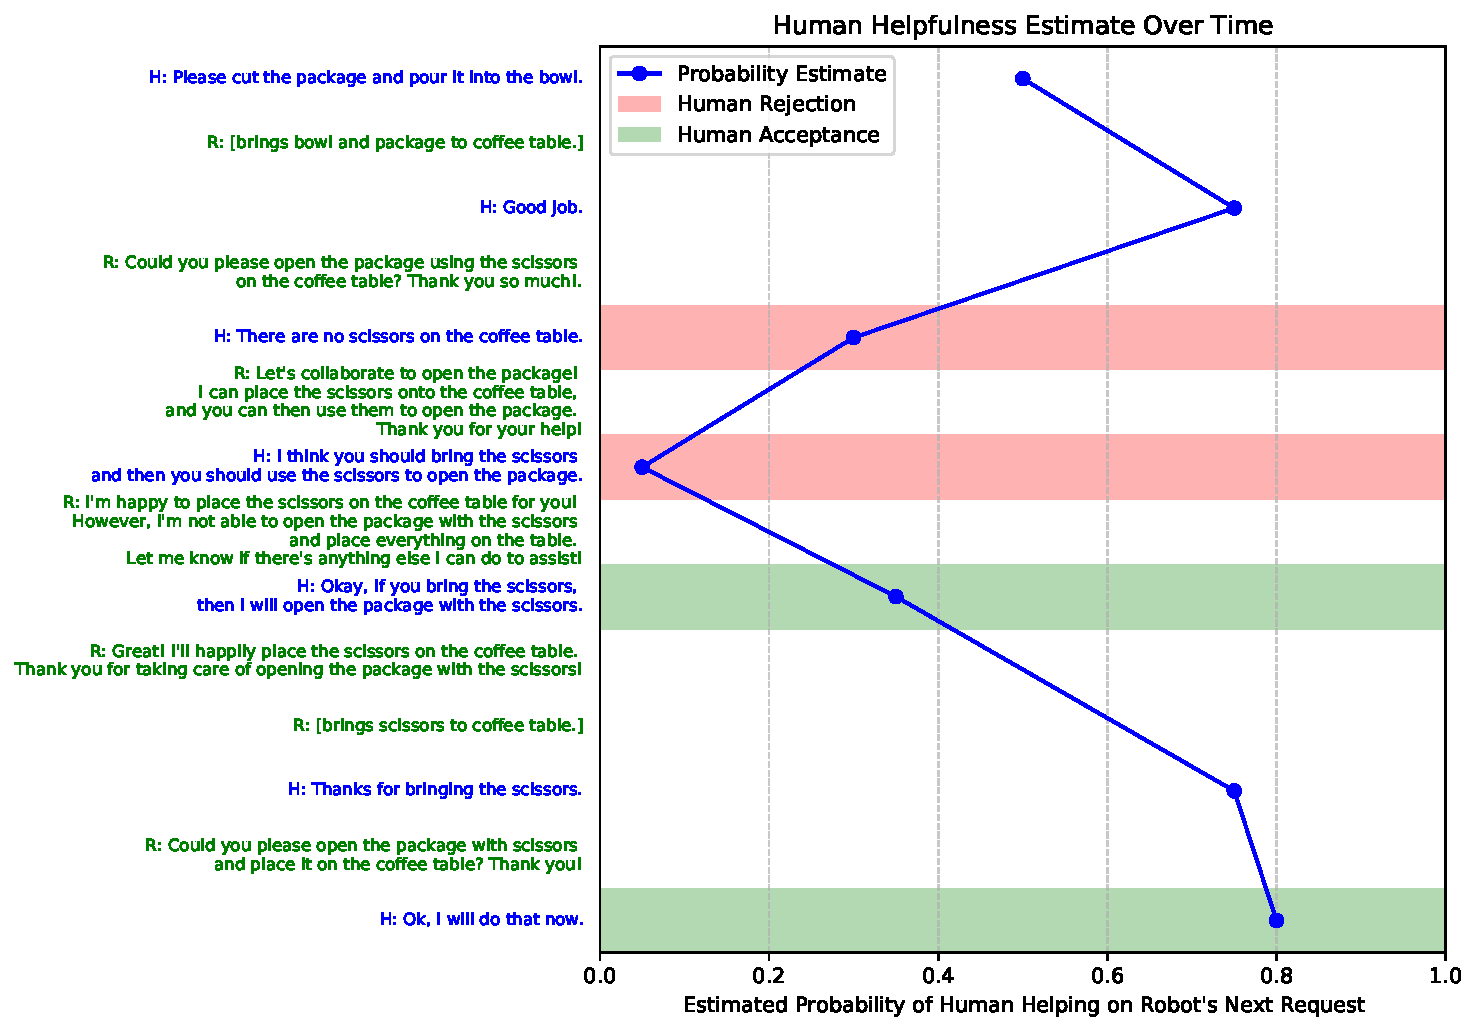
\includegraphics[width=1\textwidth,trim={0 0.0cm 0 0},clip]{figs/p_help_trial_plot.pdf}
    \caption{From a real-world user study: \ours{}'s $p_{H, t}$ estimation (blue line) reacts in real time to the human's rejections (red), acceptances (green), and encouraging remarks. All dialog is shown as $y$-labels. Green text denotes robot actions/dialog, and blue text denotes human dialog. The timestep $t$ increases from top to bottom on the $y$-axis. 
    }
    \label{fig:p-help-plot-trial}
\end{figure*}

First, we examine in Fig.~\ref{fig:p-help-plot-trial} a real-world instance of how well \ours{} can estimate the probability of the human helping on the next turn during the course of a user study. After the robot's help request was rejected twice in a row (top 2 red horizontal stripes), the robot's helpfulness estimate of the human plummets to $0.05$ (5\% estimated likelihood of the human helping the robot). However, after the robot explains its incapacity to use scissors, the human accepts the next two help requests (in green) and the robot's helpfulness estimate of the human increases to $0.8$. Note that simple comments from the human, such as a ``Thank you'' or ``good job,'' also had positive effects on the estimated $p_{H, t}$, because the robot inferred that the human was in a more positive mood and hence more likely to help. This graph demonstrates that \ours{} is fairly competent at estimating a reasonable $p_{H, t}$ value when calculating the human q-values for each step in the plan.

To analyze the effect of a good $p_{H, t}$ estimate on task allocation, we demonstrate through a controlled toy-setting in simulation in Table~\ref{tab:sim-alloc-switch} exactly how the optimal task allocation changes as the robot discovers more information about the human's willingness to help. Steps that are optimally allocated to the human are shown in \colorbox{LightBlue}{blue}, and steps optimally allocated to the robot are shown in \colorbox{LightGreen}{green}. The Q-values of the selected agent in each cell are shown in parentheses. Table~\ref{tab:sim-alloc-switch} depicts a rollout on the open and pour package into bowl (Task 1) in simulation, which has the same 5 step plan as the real-world Task 1 described in \ref{app:task-description}. Unlike our real-world experiments, where $\alpha=10$, in Table~\ref{tab:sim-alloc-switch}) we set $\alpha=0.3$ for illustrative purposes, which sets human effort to be around $3\times$ \textit{cheaper} than robot effort. In this toy setting, we program the human to reject the robot's first help request but to help the robot when it asks a second time.

Initially ($t=0$) all steps are allocated to the human. When the human rejects the initial help request from the robot, the $p_{H, t}$ estimate drops to $0.25$, increasing the Q-values of the human and switching the allocation of all but steps 2-3 to the robot after just two environment timesteps ($t=2$). (Recall that the robot cannot perform step 3, and due to the hierarchical structure of our plan, steps 2 and 3 are bundled together as an abstract step.) This demonstrates that having a good $p_{H, t}$ estimate is crucial to adapt to the human's willingness to help. Since the human demonstrated initial unwillingness to help, \ours{} quickly learns to decrease its $p_{H, t}$ estimate and allocate many more steps to itself by the second timestep. Had \ours{} not properly estimated $p_{H, t}$, the robot would have repeatedly asked the human for help even if the human was extremely unwilling to, leading to worse user satisfaction in working with the robot.

\begin{table}
\caption{Computed Best Task Allocation (and Agent Q-values) During a Sim Trial on Task 1.}
\label{tab:sim-alloc-switch}
\centering
\resizebox{\columnwidth}{!}{
\begin{tabular}{c|c|c|c|c|c}
Env. Timestep & Step 1 & Step 2 & Step 3 & Step 4 & Step 5 \\
\hline
$t=0$ & \cellcolor{LightBlue}H (-9.6) & \cellcolor{LightBlue}H (-7.2) & \cellcolor{LightBlue}H (-13.2) & \cellcolor{LightBlue}H (-2.4) & \cellcolor{LightBlue}H (-2.4) \\
$t=2$ & \cellcolor{LightGreen}R (-13.0) & \cellcolor{LightGreen}R (-9.0) & \cellcolor{LightBlue}H (-13.2) & \cellcolor{LightBlue}H (-4.8) & \cellcolor{LightGreen}R (-1.0) \\
$t=6$ & -- & \cellcolor{LightGreen}R (-12.0) & \cellcolor{LightBlue}H (-13.2) & \cellcolor{LightBlue}H (-4.8) & \cellcolor{LightGreen}R (-1.0) \\
$t=9$ & -- & -- & \cellcolor{LightBlue}H (-13.2) & \cellcolor{LightBlue}H (-4.8) & \cellcolor{LightGreen}R (-1.0) \\
$t=16$ & -- & -- & -- & -- & \cellcolor{LightGreen}R (-3.0) \\
\hline
\end{tabular}
}
\end{table}

\subsection{Meta-planner and $p_{H}$ Estimator Accuracy}
We tested LLM-generated meta-planner programs against manually-annotated ground truth in 6 user studies (3 successful + 3 failed rollouts; 59 programs total). The meta-planner achieved an \textbf{$\mathbf{89.8\%}$ accuracy (53/59 programs)}.
% In terms of producing complete and consistent programs (\reva{-Q3}{}), we did not observe any instances of an incomplete program of these 59 programs, and during metaplanning, we requery the metaplanner if the generated code does not execute (up to a maximum of 3 attempts), which helps ensure consistency.

We also tested \ours{}'s accuracy at estimating the likeliness of human helping, $p_{H, t}$. Across 33 estimates from the same 6 user studies, \ours{}'s mean absolute error (MAE) against a ground-truth (proportion of human-accepted help requests so far in the trial) was 0.11 (on a scale of 0 to 1.0). \textbf{76\% of estimates were within 0.15 of the ground truth.}
% We examined 33 estimates from the same 6 real-world user studies.
% Our method only updates the $p_{H, t}$ estimate after the human has said something.
% We computed a ``ground-truth'' value equal to the proportion of all robot help requests the human accepted so far. \uline{MicoBot's mean absolute error (MAE) was $0.113$} (MAE $\in [0, 1.0]$). \uline{$75.8\%$ of the estimates were within $0.15$ of the ground truth.}
% and $84.8\%$ were within $0.2$ of the ground truth.}

\subsection{Further Connections to Prior Work}
\label{app:extra-related-work}
\subsubsection{Agents with Both Physical and Verbal Actions}
\methodname{} relies on a heterogeneous action space that includes interacting with the physical world \textit{and} generating freeform dialogue to a human collaborator. 
Prior works have developed \textbf{policies with a combined physical and verbal action space} through RL~\cite{Das2017ICCV, shervedani2024multimodalreinforcementlearningrobots}
or IL (imitation learning)~\cite{padmakumar2022teach, deepmindinteractiveagentsteam2022creatingmultimodalinteractiveagents}. 
Research on language emergence in multiagent systems~\cite{Peters_2025, kottur-etal-2017-natural} has also examined how cooperative agents learn to communicate through latent representations or natural language when performing simulated robotic tasks~\cite{lin2021learninggroundmultiagentcommunication, lowe2020interactionsupervisionselfplayemergent, woodward2019learninginteractivelylearnassist, lobostsunekawa2022madreamercoordinationcommunicationshared, kolb2019learningrequestguidanceemergent}. However, these works are typically limited to simulated domains, where action spaces and task dynamics are highly abstracted or simplified. They often rely on limited communication protocols without integrating grounded task structure, rich human preferences, or real-world execution constraints.
In contrast, \methodname{} leverages an LLM to generate freeform, grounded dialog within a shared task context, enabling fluid mixed-initiative interaction and reasoning over both verbal and physical actions in real-world scenarios.

\subsubsection{Natural Language and Robotics}
Our work sits at the broad, growing intersection of natural language and robot learning. We refer the reader to various lines of work upon which different modules of our method are based, including language-conditioned robot policies~\cite{jang2021bc, lynch2021language, calvin2021, hulc22, shao2020concept, sodhani2021multi, silva2021langcon, karamcheti2021lila, jiang2022vima, shah2023mutex, yu2022deltaco}, LLMs as task planners~\cite{huang2022inner, saycan2022arxiv, chen2022nlmapsaycan, raman2023cape}, code-based policies~\cite{codeaspolicies2022, pmlrv235li24ar, huang2023voxposercomposable3dvalue}, hierarchical policies~\cite{shi2025hirobotopenendedinstruction, shi2024yellrobotimprovingonthefly, belkhale2024rthactionhierarchiesusing} and planners~\cite{choi2025reactree, luo2023obtaining}, vision-language representations~\cite{radford2021learning, zhai2021lit, zhu2023languagebind} for robotic control~\cite{nair2022r3m, shridhar2021cliport, shridhar2022peract, yu2024lang4sim2real}, and language-based reward shaping for RL policies~\cite{nair2021lorel, goyal2019learn, goyal2020pixl2r, fan2022minedojo, ma2023liv, ma2024eurekahumanlevelrewarddesign, ma2024dreureka, yu2023languagerewardsroboticskill}.
